
\documentclass[11pt,fleqn]{article} 
\usepackage[margin=0.8in, head=0.8in]{geometry} 
\usepackage{amsmath, amssymb, amsthm}
\usepackage{fancyhdr} 
\usepackage{palatino, url, multicol}
\usepackage{graphicx, pgfplots} 
\usepackage[all]{xy}
\usepackage{polynom} 
%\usepackage{pdfsync} %% I don't know why this messes up tabular column widths
\usepackage{enumerate}
\usepackage{framed}
\usepackage{setspace}
\usepackage{array,tikz}

\pgfplotsset{compat=1.6}

\pgfplotsset{soldot/.style={color=black,only marks,mark=*}} \pgfplotsset{holdot/.style={color=black,fill=white,only marks,mark=*}}


\pagestyle{fancy} 
\lfoot{}
\rfoot{FE Review Probs (day 1)}

\begin{document}
\renewcommand{\headrulewidth}{0pt}
\newcommand{\blank}[1]{\rule{#1}{0.75pt}}
\newcommand{\bc}{\begin{center}}
\newcommand{\ec}{\end{center}}
\renewcommand{\d}{\displaystyle}

\vspace*{-0.7in}

%%%%%%%%%intro page
\begin{center}
  \large
  \sc{Practice for the Final Exam (Day 1)}\\
  
\end{center}

\begin{enumerate}
\item Let $R$ be the region bounded by the graph of $f(x) = 1 +
  \sqrt{x}$, $g(x) = e^{-3x}$ and the vertical line $x = 1$. Sketch the region $R$.
  \begin{enumerate}
  \item Set up, but do not solve, an integral that gives the area of
    $R$.
  \item Set up, but do not solve, an integral that finds the volume of
    the solid when $R$ is rotated about the $x$-axis. 

  \item Set up, but do not solve, an integral that finds the volume of
    the solid when $R$ is rotated about the line $y$-axis. 
  \end{enumerate}
  
\item Evaluate the following integrals. 

\begin{enumerate}
\item $\d \int \sin^5 ( 2 x ) \cos^2 (2 x ) dx$
\item $\d \int \frac{2x^2 + 3x - 2}{x^3 - x^2} dx$
\item $\d \int \tan^{-1}  \left( \frac{x}{2} \right) dx$ 
\item $\d \int \frac{x^2}{(4 - x^2)^{3/2}} dx$
\end{enumerate}

\item Let $\d a_n = \ln \left( \frac{2n^2 + 1}{3n^2 + 4} \right)$.

  \begin{enumerate}
  \item Determine whether the sequence $a_n$ converges. If it is
    convergent determine what it converges to.
  \item Determine whether the series $\d \sum_{n=1}^{\infty} a_n$ converges or
    diverges. 
  \end{enumerate}
  
 \item Determine if the series below converge or diverge. Full credit
  will only be given for answers that include (1 pt) the name of the
  test being applied, (5 pts) a complete application of the test,
  including evidence that the conditions have been met, and (1 pt) a
  clear conclusion with justification.
  
  \begin{enumerate}
  \item $\d \sum_{n=1}^{\infty} \frac{n^2 + 1}{2n^3 + 2}$

  \item $\d \sum_{n=1}^{\infty} \frac{ \sin(3n) }{2 + n^4}$
  
  \item $\d \sum_{n=1}^{\infty} \frac{(-1)^n}{\sqrt{n+1} + \sqrt n}$

  \item $\d \sum_{n=2}^{\infty} \frac{1}{n (\ln n)^{3/2}}$


  \end{enumerate}

\item Find the sum of the following series exactly. 

  \begin{multicols}{2}{
      % make sure you added \usepackage{enumerate}
      \vspace*{-0.45in}
      \begin{enumerate}[a)]
      \item $\d \sum_{n = 1}^{\infty} (-3)^{n+1}5^{-n}$
      \item $\d \sum_{n = 0}^{\infty} \frac{(-1/2)^n }{n!}$
      \end{enumerate}}
  \end{multicols}
  \end{enumerate}
  \end{document}
  
  \item  Find the Taylor series for the function $f(x) = \sin(x)$ centered at $a=\pi.$
\item 
  \begin{enumerate}
  \item Determine whether the improper integral $\d \int_1^{\infty} x
    e^{-x^2} dx$ converges or diverges. Evaluate it if it is convergent.

  \item Use the integral test, and your answer from (a), determine whether $\d
    \sum_{n=1}^{\infty} n e^{-n^2} $ converges or diverges. You must
    explicitly verify that the integral test applies to this
    series. No credit will be given if another test is used. 
  \end{enumerate}
\item Determine whether the following series converge or
  diverge. You must clearly explain your reasoning. 
  \begin{enumerate}
  \item $\d \sum_{n=1}^{\infty} \frac{\sqrt n}{2n +3}$

  \item  $\d \sum_{n=1}^{\infty} (-1)^n \frac{\sqrt n}{2n +3}$

  \item Using your answers to (a) and (b), determine whether the
    series $\d \sum_{n=1}^{\infty} (-1)^n \frac{\sqrt n}{2n +3}$ is
    conditionally convergent or absolutely convergent. Explain your
    reasoning. 
\vfill
  \end{enumerate}

\item Find the radius of convergence and the interval of convergence
  of the following series. 

  \begin{enumerate}
  \item $\d \sum_{n=1}^{\infty} n! ( 2x - 1)^n$
  \item $\d \sum_{n=1}^{\infty} \frac{(x-a)^n}{n b^n}$, where $a$ and
    $b$ are positive constants.
  \end{enumerate}



\item Consider $x = t^2 + 1$, $y = e^{2t} - 1$. 
  \begin{enumerate}
  \item Find $\d \frac{dy}{dx}$.
  \item Determine the location of any vertical tangents. If none
    exist, explain why. 
  \item Find $\d \frac{d^2 y}{dx^2}$.
  \item Determine the values of $t$ for which the curve is concave
    up. 
\vfill
  \end{enumerate}
\item Consider the curve $r = 1 + 2 \cos \theta$. 
  \begin{enumerate}
  \item Sketch the curve $r = 1 + 2 \cos \theta$.
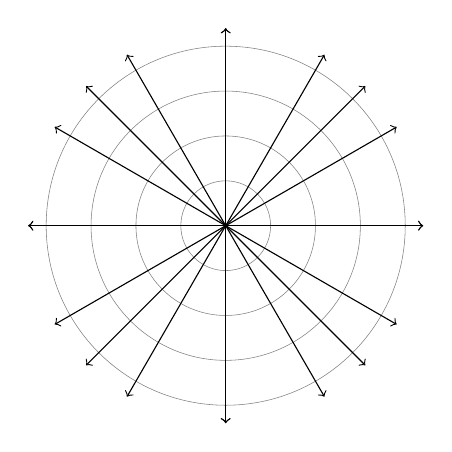
\begin{tikzpicture}[scale=0.57,baseline=(current bounding
        box.center)]
        \foreach \i in {1,2,3,4}{ \draw[help lines] (0,0) circle (\i)
          ; }

        %\foreach{\i} in {1,2,3,4}{ \draw (\i, 0) node[below
          %right]{\i}; \draw (0,\i) node[above right] {\i}; }

        \foreach \i in {30, 60, ..., 360} \draw[->] (0,0) -- (\i:4.4);

        \foreach \i in {45, 90, ..., 360} \draw[->] (0,0) -- (\i:4.4);
      \end{tikzpicture}


  \item Find the area enclosed by the inner loop.
 
  \end{enumerate}
  
  \item  Let $\mathcal{R}$ be the region bounded by $y = e^x$ and $y =
  0$, $0 \le x \le 2$. 
  \begin{enumerate}
  \item Sketch the region and find the area of $\mathcal{R}$.
  \item Find the centroid of the the region $\mathcal{R}$. 
  \end{enumerate}
  
  \end{enumerate}

\end{document}

